% !TEX TS-program = pdflatex
% !TEX encoding = UTF-8 Unicode
% arara: pdflatex: { synctex: true }
\pdfminorversion=7
% \PassOptionsToPackage{rgb,svgnames,dvipsnames,x11names}{xcolor}
\documentclass[tikz,border=10pt]{standalone}
\usetikzlibrary{automata,positioning,arrows.meta}

\begin{document}
  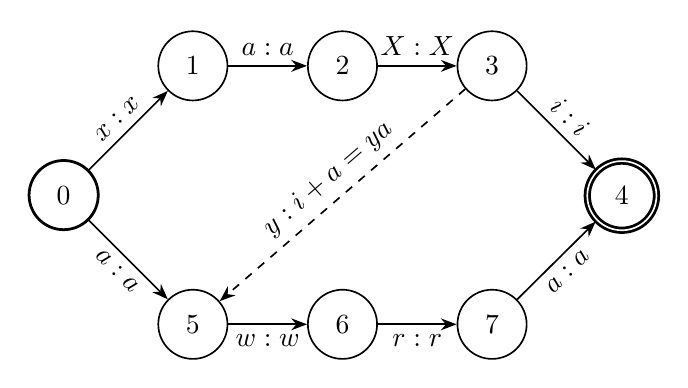
\begin{tikzpicture}
	[
	  initial/.style={line width=1pt},
	  accepting by double/.append style={line width=1pt},
	  semithick,
	]
	\node (0) [state, initial] {$0$};
	\node (1) [state, above right=of 0] {$1$};
	\node (2) [state, right=of 1] {$2$};
	\node (3) [state, right=of 2] {$3$};
	\node (5) [state, below right=of 0] {$5$};
	\node (6) [state, right=of 5] {$6$};
	\node (7) [state, right=of 6] {$7$};
	\node (4) [state, below right=of 3, accepting] {$4$};
	\path [-{Stealth[]}]
	  (0) edge node [above, sloped] {$x:x$} (1)
		edge node [below, sloped] {$a:a$} (5)
	  (1) edge node [above] {$a:a$} (2)
	  (2) edge node [above] {$X:X$} (3)
	  (3) edge node [above, sloped] {$i:i$} (4)
	  (5) edge node [below] {$w:w$} (6)
	  (6) edge node [below] {$r:r$} (7)
	  (7) edge node [below, sloped] {$a:a$} (4)
	  (3) edge [dashed] node [above, sloped] {$y:i+a=ya$} (5)
	  ;
  \end{tikzpicture}
\end{document}
